\documentclass[letterpaper,12pt]{texMemo}

\usepackage{graphicx}

\memoto{Bonnie Hsia, Prof SJSU}
\memofrom{Partha Sarathi Ghosh}
\memosubject{Literature Review Progress Report}
\memodate{\today}
%\logo{\includegraphics[width=0.3\textwidth]{Microsoft-Logo.pdf}}

\begin{document}
\maketitle

%In the opening paragraph of your memo or email, you should always tell your reader why he or she is receiving this email in particular and what the purpose is for the email. What this means is that your opening paragraph will probably be fairly short, possibly no more than one sentence or two.
\noindent This memo is a progress report for the Literature Review assignment in ENGR-200W course.

%%%%%%%%%%%%%%%%%%%%%%%%%%%%%%%
%PARTHA'S section starts here
%%%%%%%%%%%%%%%%%%%%%%%%%%%%%%%

\section*{Summary}
%This paragraph provides a brief overview of the issue that is being discussed in the memo, and it should contain a summary of your recommendations and conclusions. When readers are busy, they will often only read the summary, and so providing this section is important. The summary usually will be longer than the opening paragraph, but will generally only be one paragraph for a one to two page-memo. (Note that for a summary may be unnecessary for a memo that is shorter than one page.)
%
This memo is written to provide an update about my Master's thesis work. It contains a brief summary and rational for selecting the topic for the thesis. It also briefly describes the goal, work items, advisors and choice of literature style for the thesis work.
%%%%%%%%%%%%%%%%%%%%%%%%%%%%%%%
%PARTHA'S section starts here
%%%%%%%%%%%%%%%%%%%%%%%%%%%%%%%

\section*{Discussion}
%This section will usually be two paragraphs long. The first paragraph will pull together what you’ve had to say in your memo/email, and the second paragraph will put what you’ve said into the context of an ongoing dialog with your reader. An example of this might be a something like, “Thank you in advance for taking the time to consider this important issue; I’ll be calling your office next week to find out when a mutually convenient time is to meet for us to discuss it with you.”
%
%Here is some final advice to consider.
%\
%•	As you plan your writing, take length into account. Note, for example, that this memo is 913 words long.
%•	When you start to write, begin with writing the discussion section first, then the conclusions and the summary, and finally, the opening paragraph.
%•	Make sure that you save at least five to ten minutes at the end of a lab period to review what you have written and to edit it.
%
%I appreciate the time that you are taking to review the contents of this memo. Please feel free to email me if you have any questions or to bring them up in class.
%

%%%%%%%%%%%%%%%%%%%%%%%%%%%%%%%
%PARTHA'S section starts here
%%%%%%%%%%%%%%%%%%%%%%%%%%%%%%%
% Trial project topic : Asset Vulnerability Ranking Algorithm for Security Risk Management
% Rational for Topic : Risk Management is one the primary tools used in Cyber security today. Risk Management involves identifying all the physical and virtual assets in any organization, followed by assigning risk profile to each asset and finally perform the task of Risk Mitigation. The software and hardware assets could be physically or virtually distributed across geographies. All computing hardware and software resources are interconnected in an enterprise network infrasturecture. Manually inventroising these assests are a humongous task in itself.
% The soope of this topic would be to perform 3 things
% Identify the methods to aggregate the information on the availability of the hardware and software assets in an enterprise network
% Identify the parameters that would be used in identifying the vulnerablity of a system
% Study different stochastic methods to be used in the creation of the algorithm
% Explore the possibility of creating a vulnerability ranking aglorithm for these assets based on their hardware configurations, operating systems, open source software being used and other parameters
%
% Advisor : My advisor for this project are Steve Turner, Ph.D., Senior Director, Cumulus Networks,
% Prof. KaiKai Liu, Ph.D., San Jose State University
%
% Anicipated Graduation data : my anticipated date of graduation December 2020.
% Citation sytle : I will be using IEEE citation style as that is the standard sytle recommended by Office of Graduate Studies at San Jose State University.


\noindent The title of my thesis is \textit{Asset Vulnerability Ranking Algorithm for Security Risk Management}. Risk Management is one the primary tools used in cyber security today. Risk Management involves the following steps on the assets.
 \begin{enumerate}
     \item Identify all the physical and virtual assets in an organization.
     \item Assign a risk profile to each asset.
     \item Perform risk evaluation on each asset.
     \item Perform risk mitigation on each asset.
 \end{enumerate}

\noindent The software and hardware assets in an organization could be physically or virtually distributed across geographies. All computing hardware and software resources are interconnected in an enterprise network infrastructure. Manually inventorying these assets are a humongous task in itself. One of the approach to minimize the security risks in an organization is to perform a risk assessment on these assets.

The scope of this topic would be to achieve the following 4 objectives,

\begin{enumerate}
    \item  Identify the methods to aggregate the information on the hardware and software assets in an enterprise network.
    \item  Identify the parameters that would be used in identifying the vulnerability of a software or a hardware.
    \item  Study different stochastic methods to be used in the creation of the algorithm.
    \item  Explore the possibility of creating a cyber asset vulnerability ranking algorithm for these assets, based on their hardware configurations, operating systems, open source software being used and other parameters.
\end{enumerate}

\noindent My advisors for this thesis are
\begin{itemize}
   \item  Dr. Younghee Park, Ph.D. San Jose State University,
   \item  Prof. KaiKai Liu, Ph.D. San Jose State University,
   \item  Mr. Vikrant Nanda, M.S, MBA, Adjunct Prof. School of Business, SJSU,
\end{itemize}

\noindent My anticipated graduation date is December 2020. I will be using IEEE style for citation, as that is the style recommended by the Office of Graduate Studies at San Jose State University. \\

\noindent I have created a schedule using Gantt chart for this thesis work. The Gantt chart will layout my plan of work for the thesis, dividing the work into multiple tasks. \\
%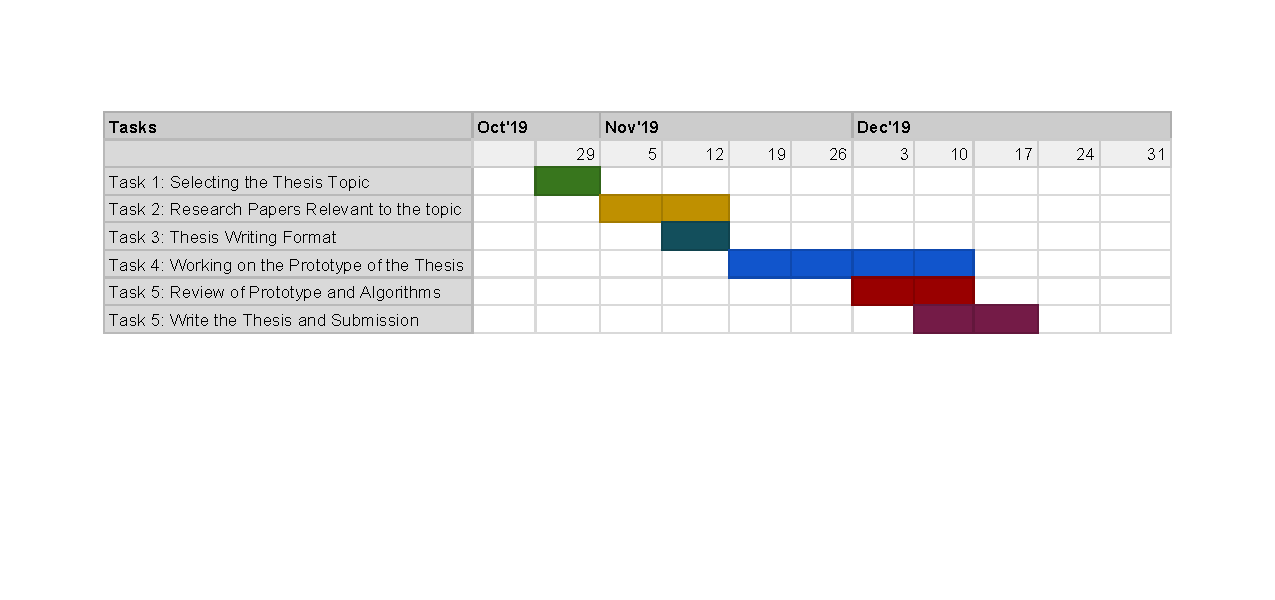
\includegraphics{GaantChartThesis.pdf}

\begin{figure}[h!]
    \centerline{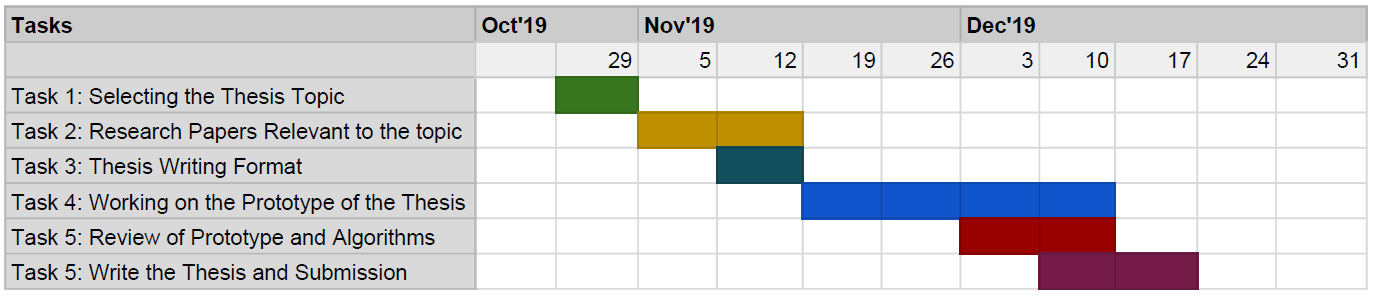
\includegraphics[scale=.45]{GaantChartThesis.PNG}}
    \caption{Gantt Chart for Litearture Review}
    %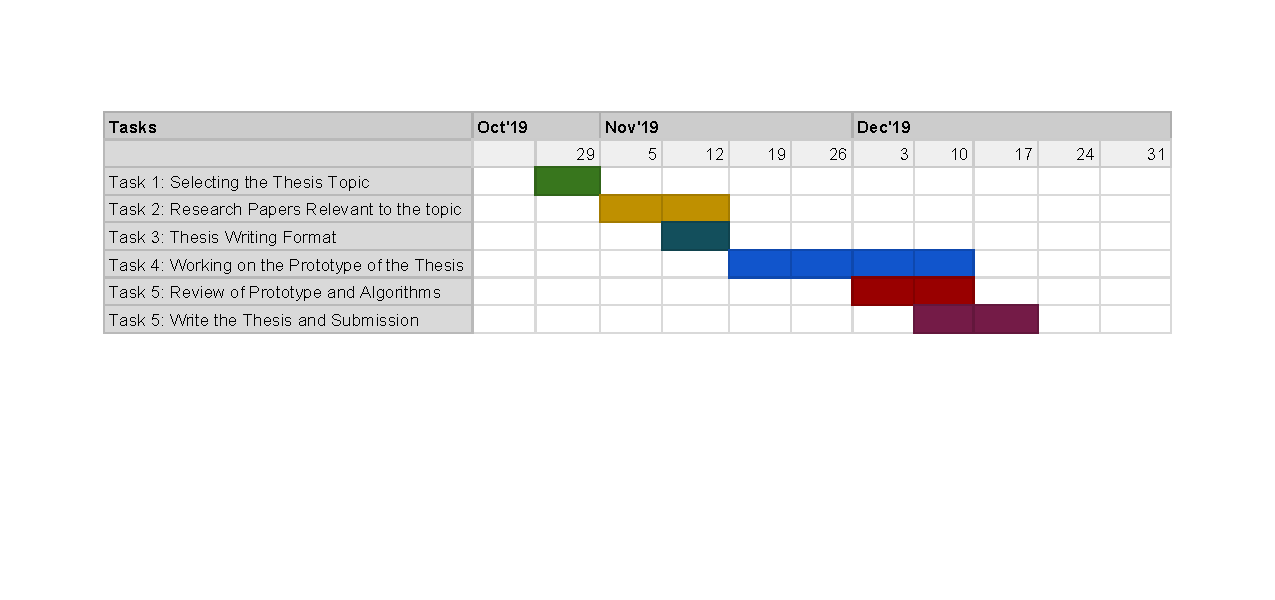
\includegraphics[scale=.8]{GaantChartThesis.pdf}
\end{figure}

\section*{Conclusion}
%This section will usually be two paragraphs long. The first paragraph will pull together what you’ve had to say in your memo/email, and the second paragraph will put what you’ve said into the context of an ongoing dialog with your reader. An example of this might be a something like, “Thank you in advance for taking the time to consider this important issue; I’ll be calling your office next week to find out when a mutually convenient time is to meet for us to discuss it with you.”
%
%Here is some final advice to consider.
%
%•	As you plan your writing, take length into account. Note, for example, that this memo is 913 words long.
%•	When you start to write, begin with writing the discussion section first, then the conclusions and the summary, and finally, the opening paragraph.
%•	Make sure that you save at least five to ten minutes at the end of a lab period to review what you have written and to edit it.
%
%I appreciate the time that you are taking to review the contents of this memo. Please feel free to email me if you have any questions or to bring them up in class.

%%%%%%%%%%%%%%%%%%%%%%%%%%%%%%%
%PARTHA'S section starts here
%%%%%%%%%%%%%%%%%%%%%%%%%%%%%%%

\noindent I'm at the early stages of research with my thesis. I'm spending time to research relevant articles, using the IEEE and ACM online library. This will help me in attaining the goals of my thesis. I'm having discussion with my professors on the different approaches that the algorithms could take to make this thesis a fruitful one. \\ 


\noindent In the coming weeks I will start working, to develop the prototype software that would be needed for the thesis. This prototype will be eventually scaled up, during the later stages of the thesis work. \\

\noindent I appreciate the time that you are taking to review this progress report and the Gantt chart. Please feel free to email me at \textit{parthasarathi.ghosh@gmail.com} if you have any questions or bring them up in class.

\end{document}
